\documentclass{beamer}

% Theme
\usetheme{Madrid}
\usepackage{tikz}

% Packages
\usepackage{graphicx}

%-------------------------------------------------
% Title Page Details
%-------------------------------------------------
\title{\textbf{Mathematics for Computing}}
\subtitle{Assignment 1}

\author{%
Poojitha Santhosh \\[0.3cm]
Department of Computer Science and Engineering with Artificial Intelligence and Software Engineering \\[0.2cm]
 }

\institute{
CUSAT
}

\date{\today}

%-------------------------------------------------
\begin{document}

%-------------------------------------------------
% Title Slide
%-------------------------------------------------
\begin{frame}
    \titlepage
\end{frame}



%-------------------------------------------------
% Slide 2
%-------------------------------------------------
\begin{frame}{Content}
\begin{itemize}
    \item Cardinality of set
    \item Types of Set in AI and DS
    \item Examples of Sets in Set Builder form
    \item Inclusion Exclusion Principle
    \item Partially Ordered Sets(Posets)
    \item Hasse Diagram Examples
\end{itemize}
\end{frame}

%-------------------------------------------------
% Slide: Cardinality of a Set
%-------------------------------------------------
\begin{frame}{Cardinality of a Set}


\begin{itemize}
    \item The \textbf{cardinality of a set} is the number of elements present in the set.
    \item It is represented by the symbol \(|A|\), where \(A\) is a set.
    \item For a finite set, cardinality gives the total count of distinct elements in that set.
\end{itemize}

\vspace{0.4cm}

\textbf{Example}

Let,
\[
A=\{2,4,6,8,10\}
\]

The number of elements in set \(A\) is 5.

Therefore, the cardinality of set \(A\) is:

\[
|A|=5
\]

\end{frame}
%-------------------------------------------------
% Slide 3: Types of Sets - Finite Set
%-------------------------------------------------
\begin{frame}{Types of Sets}

\textbf{Finite Set}

\begin{itemize}
    \item A \textbf{finite set} is a set that contains a fixed and limited number of elements.
    \[
    |A|=n
    \]
\end{itemize}

\vspace{0.3cm}

\textbf{AI \& Data Science Example}

\begin{itemize}
    \item In a machine learning classification model, the output categories form a finite set.
    \item Example: A sentiment analysis model classifies reviews into:
    \[
    S=\{\text{Positive},\text{Negative},\text{Neutral}\}
    \]
    \item Since there are only three possible outcomes, \(S\) is a finite set.
\end{itemize}

\vspace{0.3cm}

\textbf{Set-builder Form}

\[
A=\{x \in U \mid P(x)\}
\]

\end{frame}

%-------------------------------------------------
% Slide 4: Types of Sets - Infinite Set
%-------------------------------------------------
\begin{frame}{Types of Sets}

\textbf{Infinite Set}

\begin{itemize}
    \item An \textbf{infinite set} is a set that contains an unlimited number of elements and cannot be completely counted.
\end{itemize}

\vspace{0.3cm}

\textbf{AI \& Data Science Example}

\begin{itemize}
    \item In Data Science, the set of possible real-valued input features in a continuous dataset can be infinite.
    \item Example: The possible temperature values recorded by an IoT sensor:
    \[
    T=\{x \mid x \in \mathbb{R}, 0 \leq x \leq 100\}
    \]
    \item Since temperature values can have infinitely many possible real values, \(T\) is an infinite set.
\end{itemize}

\vspace{0.3cm}

\textbf{Set-builder Form}

\[
A=\{x \in \mathbb{R} \mid 0 \leq x \leq \infty\}
\]

\end{frame}

%-------------------------------------------------
% Slide 5: Types of Sets - Null Set
%-------------------------------------------------
\begin{frame}{Types of Sets}

\textbf{Null Set (Empty Set)}

\begin{itemize}
    \item A \textbf{null set} is a set that contains no elements and is represented by $\emptyset$.
\end{itemize}

\vspace{0.3cm}

\textbf{AI \& Data Science Example}

\begin{itemize}
    \item In a data science dataset, a null set represents a category where no data samples are available.
    \item Example: In an image classification dataset, if no images belong to the class "Elephant":
    \[
    E=\{\text{Images labeled as Elephant}\}=\emptyset
    \]
    \item Since the set contains no elements, \(E\) is a null set.
\end{itemize}

\vspace{0.3cm}

\textbf{General Set-builder Form}

\[
A=\{x \mid x\in U \text{ and } P(x)\text{ is not satisfied}\}
\]

\[
A=\emptyset
\]

\end{frame}

%-------------------------------------------------
% Slide 6: Types of Sets - Countable Set
%-------------------------------------------------
\begin{frame}{Types of Sets}

\textbf{Countable Set}

\begin{itemize}
    \item A \textbf{countable set} is a set whose elements can be listed in a sequence and matched with natural numbers.
\end{itemize}

\vspace{0.3cm}

\textbf{AI \& Data Science Example}

\begin{itemize}
    \item In Data Science, the set of possible class labels in a classification model is countable because each category can be listed.
    \item Example: A handwritten digit recognition model has the classes:
    \[
    D=\{0,1,2,3,4,5,6,7,8,9\}
    \]
    \item Since the elements can be counted and listed, \(D\) is a countable set.
\end{itemize}

\vspace{0.3cm}

\textbf{General Set-builder Form}

\[
A=\{x \mid x=f(n),\; n\in\mathbb{N}\}
\]

\end{frame}

%-------------------------------------------------
% Slide 7: Types of Sets - Power Set
%-------------------------------------------------
\begin{frame}{Types of Sets}

\textbf{Power Set}

\begin{itemize}
    \item A \textbf{power set} is the set of all possible subsets of a given set, including the empty set and the set itself.
\end{itemize}

\vspace{0.3cm}

\textbf{AI \& Data Science Example}

\begin{itemize}
    \item In feature selection for machine learning, the power set represents all possible combinations of features that can be selected for a model.
    \item Example: If a dataset has three features:
    \[
    F=\{\text{Age},\text{Height},\text{Weight}\}
    \]
    The power set is:
    \[
    P(F)=\{\emptyset,\{Age\},\{Height\},\{Weight\},
    \{Age,Height\},\{Age,Weight\},\{Height,Weight\},\{Age,Height,Weight\}\}
    \]
\end{itemize}

\vspace{0.3cm}

\textbf{General Set-builder Form}

\[
P(A)=\{X \mid X\subseteq A\}
\]

\end{frame}

%-------------------------------------------------
% Slide 8: Types of Sets - Subset
%-------------------------------------------------
\begin{frame}{Types of Sets}

\textbf{Subset}

\begin{itemize}
    \item A \textbf{subset} is a set in which every element of one set is also present in another set.
\end{itemize}

\vspace{0.3cm}

\textbf{AI \& Data Science Example}

\begin{itemize}
    \item In machine learning, a training dataset is a subset of the complete dataset when only selected samples are used for model training.
    \item Example:
    \[
    D=\{\text{Image1, Image2, Image3, Image4, Image5}\}
    \]
    \[
    T=\{\text{Image1, Image2, Image3}\}
    \]
    \item Since every element of \(T\) belongs to \(D\),
    \[
    T\subseteq D
    \]
\end{itemize}

\vspace{0.3cm}

\textbf{General Set-builder Form}

\[
A=\{x \mid x\in B \text{ and } P(x)\}
\]

\[
A\subseteq B
\]

\end{frame}

%-------------------------------------------------
% Slide 9: Types of Sets - Equal Set
%-------------------------------------------------
\begin{frame}{Types of Sets}

\textbf{Equal Set}

\begin{itemize}
    \item Two sets are called \textbf{equal sets} if they contain exactly the same elements, irrespective of their order.
\end{itemize}

\vspace{0.3cm}

\textbf{AI \& Data Science Example}

\begin{itemize}
    \item In machine learning, two feature sets are equal if they contain the same features used for model training.
    \item Example:
    \[
    A=\{\text{Age},\text{Height},\text{Weight}\}
    \]
    \[
    B=\{\text{Weight},\text{Age},\text{Height}\}
    \]
    \item Since both sets contain the same features,
    \[
    A=B
    \]
\end{itemize}

\vspace{0.3cm}

\textbf{General Set-builder Form}

\[
A=\{x \mid P(x)\}
\]

\[
B=\{x \mid P(x)\}
\]

\[
\therefore A=B
\]

\end{frame}

%-------------------------------------------------
% Slide 10: Types of Sets - Equivalent Set
%-------------------------------------------------
\begin{frame}{Types of Sets}

\textbf{Equivalent Set}

\begin{itemize}
    \item Two sets are called \textbf{equivalent sets} if they contain the same number of elements, even if their elements are different.
\end{itemize}

\vspace{0.3cm}

\textbf{AI \& Data Science Example}

\begin{itemize}
    \item Example:
    \[
    A=\{\text{Image1},\text{Image2},\text{Image3}\}
    \]
    \[
    B=\{\text{Audio1},\text{Audio2},\text{Audio3}\}
    \]
    \item Both sets contain three elements, therefore:
    \[
    n(A)=n(B)
    \]
    \[
    A\sim B
    \]
\end{itemize}

\vspace{0.3cm}

\textbf{General Set-builder Form}

\[
A=\{x \mid P(x)\}
\]

\[
B=\{y \mid Q(y)\}
\]

\[
A\sim B \quad \text{if } n(A)=n(B)
\]

\end{frame}

%-------------------------------------------------
% Slide 11: Types of Sets - Superset
%-------------------------------------------------
\begin{frame}{Types of Sets}

\textbf{Superset}

\begin{itemize}
    \item A \textbf{superset} is a set that contains all the elements of another set and is represented as \(A \supseteq B\).
\end{itemize}

\vspace{0.3cm}

\textbf{AI \& Data Science Example}

\begin{itemize}
    \item In machine learning, a complete dataset is a superset of a smaller dataset selected for training.
    \item Example:
    \[
    D=\{\text{Image1},\text{Image2},\text{Image3},\text{Image4},\text{Image5}\}
    \]
    \[
    T=\{\text{Image1},\text{Image2},\text{Image3}\}
    \]
    \item Since every element of \(T\) is present in \(D\),
    \[
    D\supseteq T
    \]
\end{itemize}

\vspace{0.3cm}

\textbf{General Set-builder Form}

\[
A=\{x \mid x\in U\}
\]

\[
B=\{x \mid x\in A \text{ and } P(x)\}
\]

\[
A\supseteq B
\]

\end{frame}

%-------------------------------------------------
% Slide 12: Types of Sets - Singleton Set
%-------------------------------------------------
\begin{frame}{Types of Sets}

\textbf{Singleton Set}

\begin{itemize}
    \item A \textbf{singleton set} is a set that contains exactly one element.
\end{itemize}

\vspace{0.3cm}

\textbf{AI \& Data Science Example}

\begin{itemize}
    \item In machine learning, a singleton set can represent a dataset containing only one unique data sample.
    \item Example: A facial recognition system identifying one specific registered person:
    \[
    P=\{\text{Person\_ID\_101}\}
    \]
    \item Since \(P\) contains only one element, it is a singleton set.
\end{itemize}

\vspace{0.3cm}

\textbf{General Set-builder Form}

\[
A=\{x \mid x=a\}
\]

where \(a\) is the only element of the set.

\end{frame}

%-------------------------------------------------
% Slide 1: Set Builder Form Examples
%-------------------------------------------------
\begin{frame}{Set Builder Form Examples}

\textbf{1. Natural Numbers which are Multiples of 3 but not 5}

\[
A=\{x \in \mathbb{N} \mid x \text{ is a multiple of 3 and } x \text{ is not a multiple of } 5\}
\]

Example:
\[
A=\{3,6,9,12,18,21,\ldots\}
\]

\vspace{0.4cm}

\textbf{2. Set of Perfect Cubes}

\[
B=\{x \in \mathbb{N} \mid x=n^3,\; n\in\mathbb{N}\}
\]

Example:
\[
B=\{1,8,27,64,125,\ldots\}
\]

\end{frame}

%-------------------------------------------------
% Slide 2: Set Builder Form Examples
%-------------------------------------------------
\begin{frame}{Set Builder Form Examples}

\textbf{3. Natural Numbers Between 5 and 100}

\[
A=\{x\in\mathbb{N}\mid 5<x<100\}
\]

Example:
\[
A=\{6,7,8,9,\ldots,99\}
\]

\vspace{0.4cm}

\textbf{4. Positive Integers Leaving Remainder 1 When Divided by 5}

\[
B=\{x\in\mathbb{Z}^{+}\mid x=5n+1,\; n\in\mathbb{N}\}
\]

Example:
\[
B=\{1,6,11,16,21,\ldots\}
\]

\end{frame}

%-------------------------------------------------
% Slide 3: Set Builder Form Examples
%-------------------------------------------------
\begin{frame}{Set Builder Form Examples}

\textbf{5. Odd Numbers from 1 to 15}

\[
A=\{x\in\mathbb{N}\mid x=2n+1,\;1\leq x\leq15\}
\]

Example:
\[
A=\{1,3,5,7,9,11,13,15\}
\]

\vspace{0.4cm}

\textbf{6. Set of Factors of 24}

\[
B=\{x\in\mathbb{N}\mid x \text{ divides } 24\}
\]

Example:
\[
B=\{1,2,3,4,6,8,12,24\}
\]

\end{frame}

%-------------------------------------------------
% Slide 4: Set Builder Form Examples
%-------------------------------------------------
\begin{frame}{Set Builder Form Examples}

\textbf{7. Ordered Pairs Whose Sum is 5}

\[
A=\{(x,y)\in\mathbb{Z}\times\mathbb{Z}\mid x+y=5\}
\]

Example:
\[
A=\{(0,5),(1,4),(2,3),(3,2),(4,1),(5,0)\}
\]

\vspace{0.4cm}

\textbf{8. Numbers Divisible by 2 or 3}

\[
B=\{x\in\mathbb{N}\mid x\text{ is divisible by }2
\text{ or }3\}
\]

Example:
\[
B=\{2,3,4,6,8,9,10,12,\ldots\}
\]

\end{frame}

%-------------------------------------------------
% Slide 5: Set Builder Form Examples
%-------------------------------------------------
\begin{frame}{Set Builder Form Examples}

\textbf{9. Natural Numbers and Their Squares}

\[
A=\{x^2\mid x\in\mathbb{N}\}
\]

Example:
\[
A=\{1,4,9,16,25,36,\ldots\}
\]

\vspace{0.4cm}

\textbf{10. Prime Numbers from 1 to 30}

\[
B=\{x\in\mathbb{N}\mid x \text{ is prime and }1<x\leq30\}
\]

Example:
\[
B=\{2,3,5,7,11,13,17,19,23,29\}
\]

\end{frame}

%-------------------------------------------------
% Slide 1: Inclusion-Exclusion Principle
%-------------------------------------------------
\begin{frame}{Inclusion-Exclusion Principle}

\textbf{General Formula}

\begin{itemize}
    \item The Inclusion-Exclusion Principle is used to find the number of elements in the union of multiple sets by correcting the overcounting of common elements.
\end{itemize}

\vspace{0.3cm}

For three sets \(A\), \(B\), and \(C\):

\[
|A\cup B\cup C| =
|A|+|B|+|C|
-|A\cap B|
-|A\cap C|
-|B\cap C|
+|A\cap B\cap C|
\]

\vspace{0.4cm}

\textbf{General Formula for \(n\) Sets:}

\[
\left|\bigcup_{i=1}^{n} A_i\right|
=
\sum |A_i|
-\sum |A_i\cap A_j|
+\sum |A_i\cap A_j\cap A_k|
-\cdots
+(-1)^{n+1}
\left|A_1\cap A_2\cap\cdots\cap A_n\right|
\]

\end{frame}

%-------------------------------------------------
% Slide: Posets
%-------------------------------------------------
\begin{frame}{Partially Ordered Sets (Posets)}

\textbf{Brief Explanation}

\begin{itemize}
    \item A \textbf{partially ordered set (Poset)} is a set together with a relation that satisfies three properties:
    \begin{enumerate}
        \item \textbf{Reflexive:} \(a \leq a\)
        \item \textbf{Antisymmetric:} If \(a \leq b\) and \(b \leq a\), then \(a=b\)
        \item \textbf{Transitive:} If \(a \leq b\) and \(b \leq c\), then \(a \leq c\)
    \end{enumerate}
    \item A poset is represented as \((P,\leq)\), where \(P\) is a set and \(\leq\) is a partial order relation.
\end{itemize}

\vspace{0.3cm}

\textbf{Example}

\begin{itemize}
    \item Let
    \[
    P=\{1,2,3,6\}
    \]
    with the relation "divides" (\(|\)).
    
    \[
    1|2,\quad 1|3,\quad 2|6,\quad 3|6
    \]
    
    \item Therefore, \((P,|)\) forms a Poset.
\end{itemize}

\end{frame}

%-------------------------------------------------
% Example of Poset with Hasse Diagram
%-------------------------------------------------
\begin{frame}{Example of Poset: Hasse Diagram}

\textbf{Example: Divisibility Poset}

Let 
\[
P=\{1,2,3,6\}
\]

with the relation "divides" (\(|\)).

The partial order relations are:

\[
1|2,\quad 1|3,\quad 2|6,\quad 3|6
\]

The Hasse diagram of the Poset \((P,|)\) is:

\vspace{0.5cm}

\begin{center}
\begin{tikzpicture}[scale=1.2]

% Nodes
\node (6) at (0,2) {6};
\node (2) at (-1,1) {2};
\node (3) at (1,1) {3};
\node (1) at (0,0) {1};

% Edges
\draw (1)--(2);
\draw (1)--(3);
\draw (2)--(6);
\draw (3)--(6);

\end{tikzpicture}
\end{center}

\textbf{Conclusion:}
\[
(P,|) \text{ is a partially ordered set (Poset).}
\]

\end{frame}

%-------------------------------------------------
% Slide 2: Poset Hasse Diagram Example 2
%-------------------------------------------------
\begin{frame}{Example of Poset: Hasse Diagram}

\textbf{Example 2: Subset Poset}

Let,
\[
P=\{\emptyset,\{a\},\{b\},\{a,b\}\}
\]

with the relation \(\subseteq\).

The subset relations are:

\[
\emptyset \subseteq \{a\},\quad
\emptyset \subseteq \{b\},\quad
\{a\}\subseteq\{a,b\},\quad
\{b\}\subseteq\{a,b\}
\]

\begin{center}
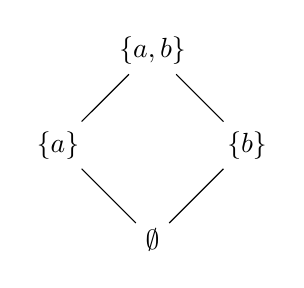
\begin{tikzpicture}[scale=1.2]

\node (ab) at (0,2) {$\{a,b\}$};
\node (a) at (-1,1) {$\{a\}$};
\node (b) at (1,1) {$\{b\}$};
\node (e) at (0,0) {$\emptyset$};

\draw (e)--(a);
\draw (e)--(b);
\draw (a)--(ab);
\draw (b)--(ab);

\end{tikzpicture}
\end{center}

\[
(P,\subseteq) \text{ is a Poset}
\]

\end{frame}

%-------------------------------------------------
% Slide 3: Poset Hasse Diagram Example 3
%-------------------------------------------------
\begin{frame}{Example of Poset: Hasse Diagram}

\textbf{Example 3: Factor Poset}

Let,

\[
P=\{1,2,3,4,6,12\}
\]

with the relation "divides" (\(|\)).

The divisibility relations are:

\[
1|2,\quad 1|3,\quad 2|4,\quad 2|6,\quad 3|6,\quad 4|12,\quad 6|12
\]

\vspace{0.3cm}

\begin{center}
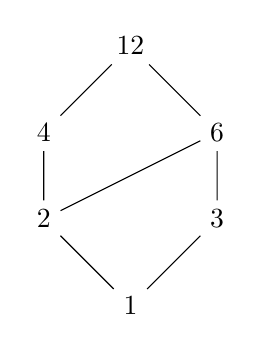
\begin{tikzpicture}[scale=1.1]

% Nodes
\node (12) at (0,3) {12};
\node (4) at (-1,2) {4};
\node (6) at (1,2) {6};
\node (2) at (-1,1) {2};
\node (3) at (1,1) {3};
\node (1) at (0,0) {1};

% Edges
\draw (1)--(2);
\draw (1)--(3);
\draw (2)--(4);
\draw (2)--(6);
\draw (3)--(6);
\draw (4)--(12);
\draw (6)--(12);

\end{tikzpicture}
\end{center}

\vspace{0.2cm}

\[
(P,|) \text{ forms a partially ordered set (Poset).}
\]

\end{frame}

\end{center}
\end{frame}

\end{document}